\documentclass[12pt,a4paper]{article}
\usepackage[ddmmyyyy]{datetime}
\renewcommand{\dateseparator}{.}
\usepackage[T1]{fontenc}
\usepackage[utf8]{inputenc}
\usepackage{graphicx} % Grafikleri eklemek için gerekli paket
\graphicspath{{images/}} % Grafik yolu belirleme
\renewcommand{\figurename}{Şekil}
\usepackage{geometry}
%\usepackage{natbib}
\usepackage{pdflscape} %Landscape format	
\usepackage[export]{adjustbox}
\renewcommand{\refname}{Kaynakça}
\title{\bf\fontsize{12pt}{14pt}\selectfont KÜTAHYA SAĞLIK BİLİMLERİ ÜNİVERSİTESİ \\ MÜHENDİSLİK VE DOĞA BİLİMLERİ FAKÜLTESİ}

\begin{document}
	\maketitle
	\thispagestyle{empty}
	\begin{center}
		
\includegraphics{images/ksbu.png}
	\end{center}
	\begin{center}
		\vspace{1cm} % Vertical space of 1cm
	\end{center}
	\begin{center}
		\title{\bf\fontsize{12pt}{14pt}\selectfont YAPAY ZEKA DERSİ }
	\end{center}
	\begin{center}
		\title{\bf\fontsize{12pt}{14pt}\selectfont İNSANLARIN KÖPEKLERDEN KORKMASINI ENGELLEME}
	\end{center}
	\begin{center}
		\vspace{1cm} % Vertical space of 1cm
	\end{center}
	\begin{center}
		
		%\title{\bf\fontsize{12pt}{14pt}\selectfont Hande Öz\hspace{1.5cm}2118121038}	
		\author{\bf\fontsize{12pt}{14pt}Hande Öz\hspace{1.5cm}2118121038}
		
		\begin{center}
			\vspace{1cm} % Vertical space of 1cm
		\end{center}
		\begin{center}
			\vspace{1cm} % Vertical space of 1cm
		\end{center}
	\end{center}
	
	\section{Giriş} 
		Bu projede, hayvanlara karşı korku duygusu besleyen insanların korkularını azaltmak veya ortadan kaldırmak için yapay zeka algoritmalarından A* algoritması ve Unreal Engine oyun motoru kullanılacaktır. A* algoritması, hayvan ile insan arasındaki mesafeyi gerçek zamanlı olarak belirlemek için kullanılırken, Unreal Engine ise bu mesafeye göre sanal bir ortam oluşturmak ve kullanıcıyı bu ortamda hayvanlarla etkileşime sokmak için kullanılması amaçlanmaktadır.
		
		
		\section{Literatür Taraması}
		\begin{enumerate}
			\item[a)] Projemize yakın olarak yapılan çalışmalar vardır 
			Bu makalede, sinofobi (köpekten korkma) tedavisinde sanal gerçeklik maruziyetine dayalı terapinin etkinliği araştırılmıştır. Özellikle, işitsel-görsel ortamların duygu ve varlık üretme etkinliği incelenmiştir.
			Sinofobi, hem görsel hem de işitsel bileşenleri olan bir fobi türüdür.Makalede, sinofobi tedavisinde sanal gerçeklik tabanlı maruz bırakma terapisinin etkisini değerlendirmek için çeşitli sanal ortamlar kullanılmıştır. Bu ortamlar, çeşitli anksiyojenik durumların simülasyonlarını içermektedir ve farklı düzeylerde görsel ve işitsel uyarıcılar içermektedir.\newline
			
			İlk Ortam: Bu sanal ortamda, bir koridor bulunmaktadır. Eğitim ortamında ağaçlar, bir ev, masalar, ve banklardan oluşan bir bahçe de bulunmaktadır.\newline
			
			İkinci Ortam: Bu ortam, büyük ve karanlık bir hangarda yer alan bir iç mekanı simüle etmektedir. Bu ortamda, farklı endüstriyel makine parçaları aktif ve gürültülü bir şekilde gösterilmektedir. Ayrıca, bu ortamlarda birkaç köpek aşamalı olarak gösterilmiştir.\newline
	
	
			 Bu projede tereoskopik Görüntüleme,3D Ses,Kafa Takip Sistemi,Kablosuz Joystick gibi teknolojiler kullanılmıştır.
			 \pagenumbering{gobble} %Sayfa numaralandırması kalkıyor
			\pagenumbering{arabic} %Sayfa numaralandırmasını bu sayadan başlat
			\setcounter{page}{1}.
			
			
			Projede, sanal gerçeklik (VR) teknolojisini kullanarak sinofobi (köpeklerden korkma) tedavisi amaçlamaktadır. Kullanıcılar, bu sanal ortamda rahatlama ve sakinleşmeyi teşvik eden işitsel ve görsel uyaranlara maruz kalmaktadır. \newline
			Bu çalışmada gerekli koşullar sağlandığında köpek korkusunun önüne geçilebileceği görülmüştür\cite{MarinaTaffou}.\newline
		
			\item[b)]  
			Bu makale bir çocuğun köpek korkusunu yenmesine yönelik bir çalışmadır.
			Bu çalışma hayvanat bahçesinde geçiyor orada sorumlu olan adam bu makalede çocuğun küçükken bir köpeğin üzerine atladığını  bu yüzden köpeklerden korktuğunu ve köpeklerin dişlerinden korktuğunu  öğreniyor.
			
			Hayvanat bahçesinde, sorumlu bir kişi çocuğun korkusunu yenmesi için ona eşlik etmiş ve 8 seansta, melez bir köpek olan Zoti ile çocuğun arasında bir bağ kurmayı başarmıştır.
			İlk seansta daha önce sırtında bir tümör olan kısa süre önce ameliyatla alınan sağlıklı bir  köpek olan zotinin hastalığını cocuk öğrenmiş ve üzülmüş köpekte çocuğun üzüldüğünü anlamış gibi iç çekmiş insan empati testlerinde başarılı olan insanlar hayvanların duygusal seslerini çözmede de ölçülebilir derecede daha iyidirler sonraki seanslarda sorumlu kişi  köpeğe uzaktan ödül maması verdirtmiş sonrasında çocuk yakınlaşarak ödül maması vermiş yeterli miktarda zaman çocuk ile köpeği aynı ortamda bulundurmuş çocuğu köpeğe adım adım yaklaştırmıştır.
			
			
			doğru köpek ve yaklaşımla köpek korkusu üstesinden gelinebilir işin püf noktası başlangıçta doğru tür köpekle eşleşmek ve hastayı zorlamamak,doğru miktarda zaman ayırmak ve onlara korkularının normal oldugunu ancak bunun sadece bir korku olduğunu ve onunla yüz yüze ilgilenerek kesinlikle yenebileceklerini göstermektedir\cite{ahsan2023deep}. \newline \newline

	\end{enumerate}
		\section{Metodoloji} 
		\begin{itemize}
			\item Unreal Engine:Unreal Engine, Epic Games tarafından geliştirilen bir oyun motorudur. Unreal Engine, oyun geliştiricilerine oyun dünyalarını oluşturmak, 3D modelleme, fizik ve animasyon gibi çeşitli özelliklerle oyunların geliştirilmesine olanak tanır. Ayrıca, sanal gerçeklik (VR) kullanılabilir. 
			\item Python:Python, kullanımı kolay,yüksek seviyeli bir bir programlama dilidir.Web geliştirme, veri analizi, yapay zeka, oyun geliştirme ve daha birçok alanda kullanılır. 
			\item Blueprint:Blueprint, Unreal Engine'in görsel programlama sistemi olarak bilinir. Geliştiricilere kod yazmadan oyun ve uygulamalar oluşturmak için bir araç sağlar. Bir kullanıcı arayüzü kullanarak, nesneler arasında ilişkiler kurabilir, etkileşimler belirleyebilir.
		     	\item Aktör/Static mesh:Static Mesh, sabit bir geometriye sahip olan nesneler için kullanılırken duvar,taş gibi.Aktörler,statik olmayan nesneleri temsil etmek için de kullanılabilir, bir oyuncu karakteri, bir ışık kaynağı gibi.
			\item Asset: Bir oyun motorunda veya dijital içerik üretim aracında kullanılan her türlü grafik, model, ses, animasyon, metin dosyası gibi içerikler asset olarak adlandırılır. Bu, oyun geliştiricilerin projelerinde kullanabilecekleri kaynak dosyalarını ifade eder.\newline 
			 Projemizde asset olarak köpek kullanacağız köpek türü olarak en az korkutucu tür ve arkadaş canlısı olan Cavalier King Charles ırkını kullanacağız.\newline\newline
			 \begin{center}
			 	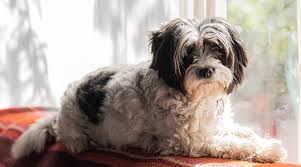
\includegraphics[width=0.7\textwidth,center]{images/images.jpeg}\newline\newline
			 \end{center}
			 
		     \begin{flushleft}
		 		Sahnede  aşağıdaki  bahçe kullanabilir.
		     \end{flushleft}
		     \begin{center}
				\includegraphics[width=0.7\textwidth,center]{images/menubackground.png}\cite{kopek}\cite{bahce}\newline
		   	\end{center}
			 
	     \end{itemize}
	
\section{Gantt Chart ve İş Akış Planı \newline} 
\begin{figure}[h] 

	\centering
	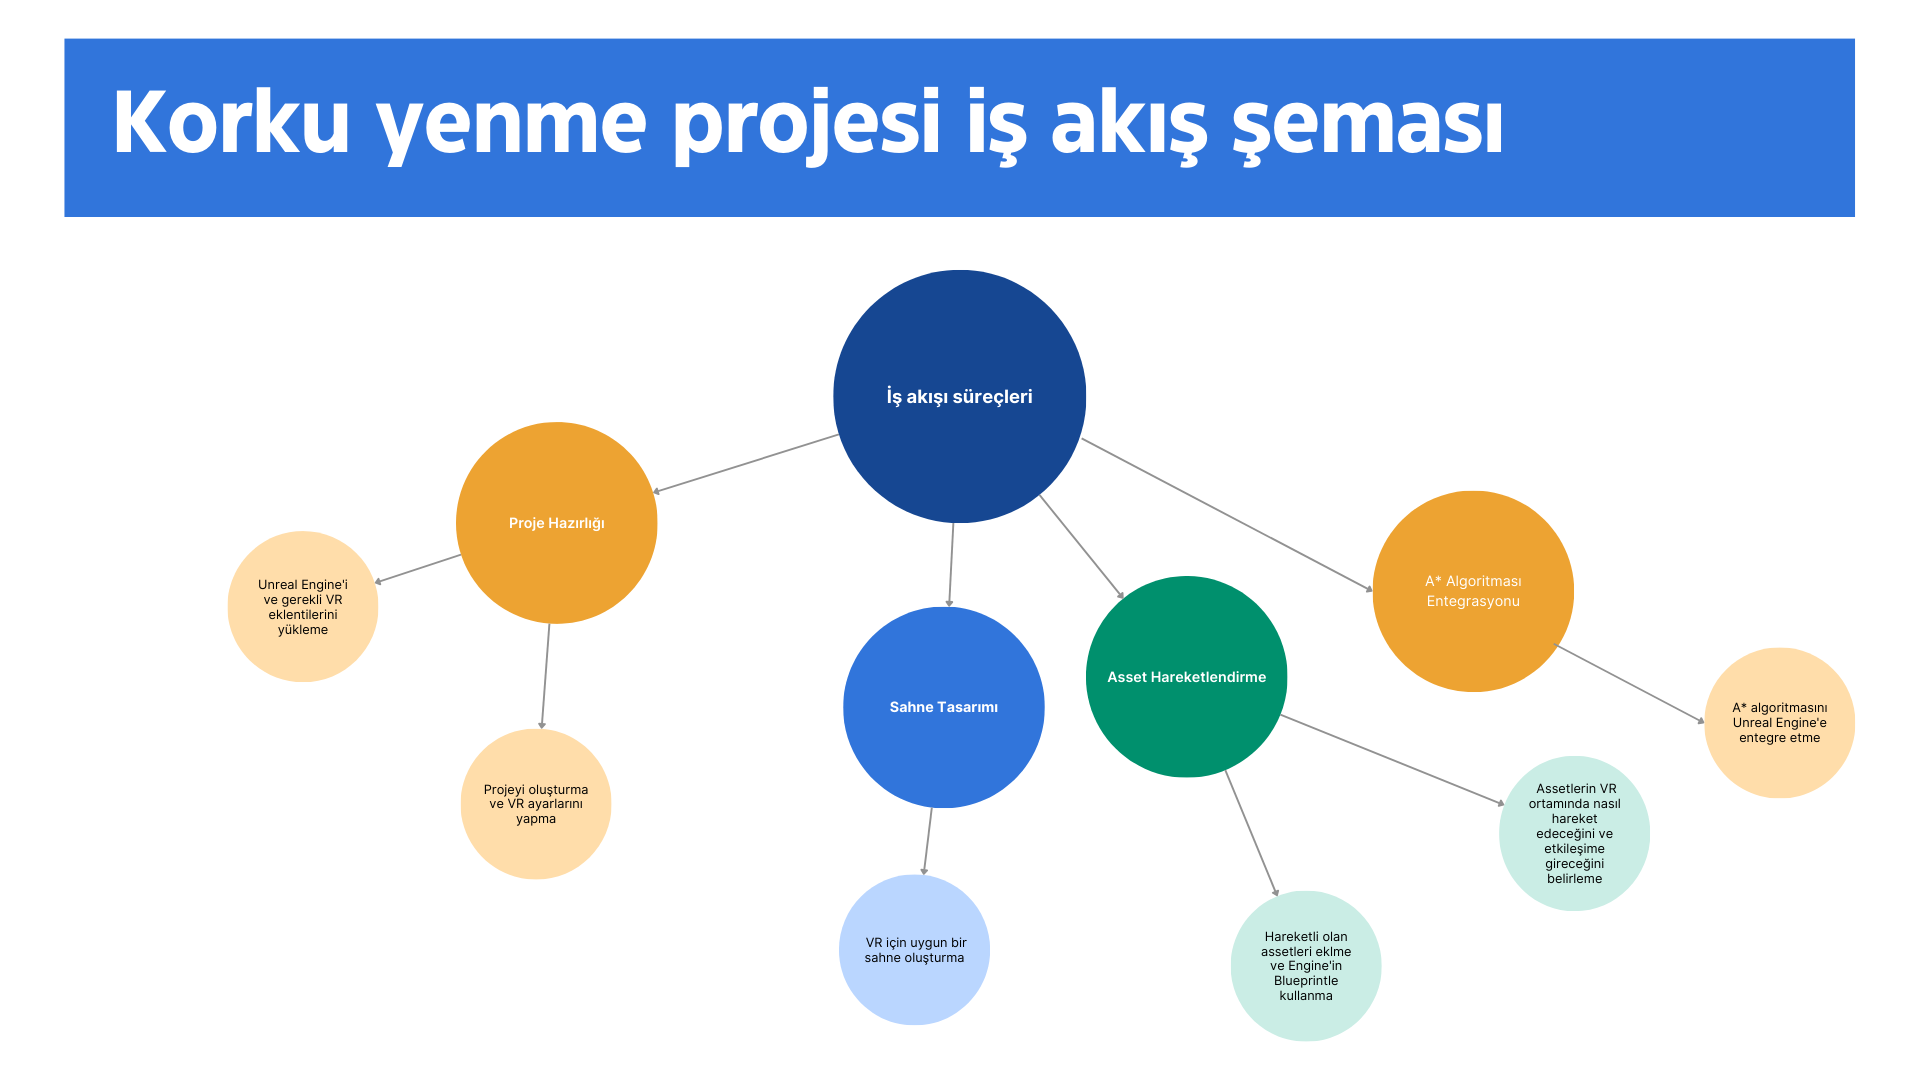
\includegraphics[width=0.9\textwidth ,height= 90mm ]{images/isakisi.png}\newline
	Projenin akış şeması yukarıdaki gibidir.
\end{figure}

%\begin{landscape}
\begin{figure}[!htbp]

	\caption{Gantt Chart}
	\centering
	%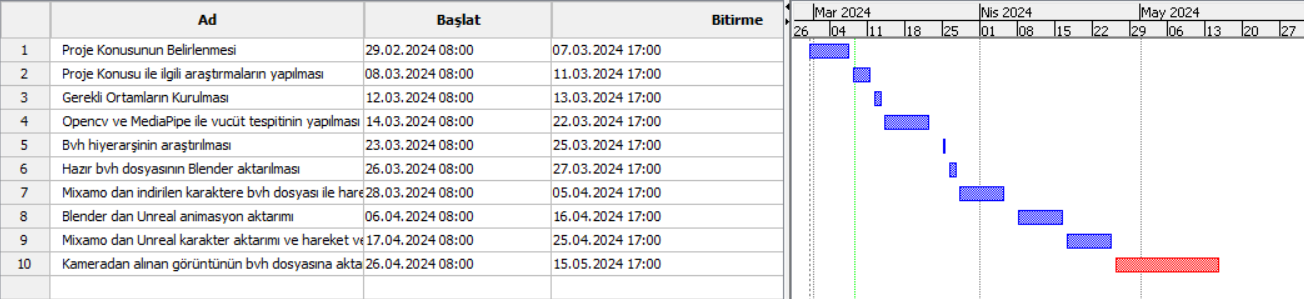
\includegraphics[angle=90, width=\textwidth]{x.png}
	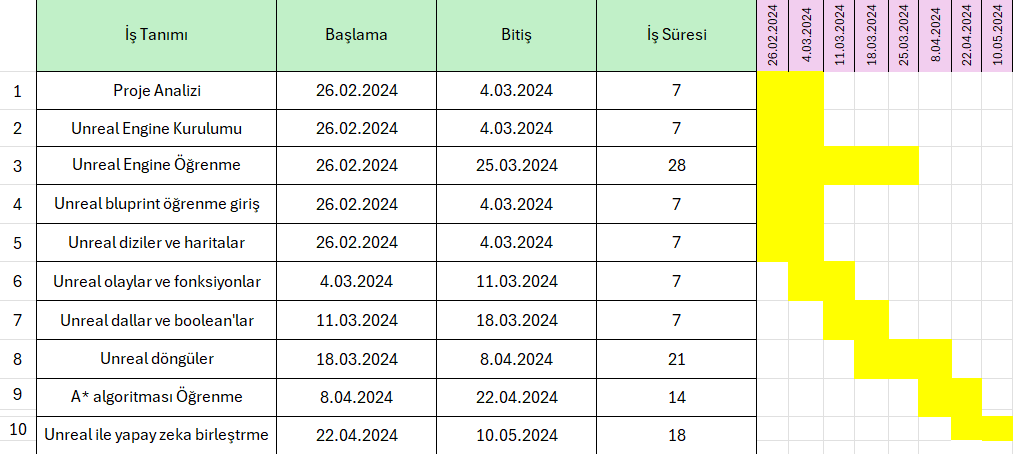
\includegraphics[height= 5 cm]{ganttchart2.png}\newline
	\label{gantt}		
\end{figure}    
     %\end{landscape}
	\newpage
		\section{Sonuç}
		Bu projede yapay zeka kullanılarak insanların köpek korkusunun önüne geçilmesi planlanmaktadır.Bu proje sayesinde insanların sokakta,köpek olan herhangi bir yerde korkusunu yenip aşırı tepki göstermemesi sonucuyla köpek saldırı vakaları azalabilir.
	\newline \newline \newline
	\bibliographystyle{ieeetr}
	\bibliography{kaynakca} 

\end{document}